\documentclass[notes=show]{beamer}

\usepackage{comment}
\usepackage{default}
\usepackage[utf8]{inputenc}
\usepackage{listings}

\definecolor{OliveGreen}{cmyk}{0.64,0,0.95,0.40}
\definecolor{Gray}{gray}{0.5}

\lstset{
    language=C,
    basicstyle=\ttfamily\scriptsize,
    keywordstyle=\color{OliveGreen},
    commentstyle=\color{Gray},
    captionpos=b,
    breaklines=true,
    breakatwhitespace=false,
    showspaces=false,
    showtabs=false,
    numbers=left,
}

\begin{document}

\begin{frame}
\frametitle{Periodic Counting Network}
\begin{itemize}
\item A parallel way of counting.
\item Replaces one bottleneck (the counter) with multiple bottlenecks.
\item Maximum throughput when the number of tokens is roughly equal to the number of 
 	  balancers in the network.
\end{itemize}
\end{frame}
\note{A note} % TODO

\begin{frame}
\frametitle{Periodic Counting Network}
\begin{itemize}
\item Principle: Given a a number of inputs $x_i$ and outputs $y_i$ and a network width $w$,
      transform an unpredictable sequence of inputs ($x_3, x_2, x_2, x_0, x_1$) into a sequential
      output sequence ($y_0, y_1, y_2, y_3, y_0$).
\item Each thread can tell its result without consulting other counters.
\item A periodic counting network consists of a sequence of identical subnetworks.
\end{itemize}
\end{frame}

\begin{frame}
\frametitle{Experience}
\begin{itemize}
\item Not much contact with pheet.
\item Difficult to integrate into my usual project setup (git, automated
      hand-in and unit tests).
\item Saturn is partly outdated,
      missing CMake files, and has components installed in odd locations.
\item Template programming requires headers-only or explicitly instantiating all
      required template instances before use.
\end{itemize}
\end{frame}
\note{
First of all, I didn't actually have much contact with pheet, so there's not too
much to say about that. \\
Integration was somewhat harder than usual because pheet doesn't use git and
I didn't want to copy the entire source tree into my repository. \\
With template programming, there was a choice of writing everything in headers only,
or instantiating the required template types somewhere. And I went with headers, simply
because it was less work to set up.
}

\begin{frame}[fragile]
\frametitle{Code}
\framesubtitle{incr()}
\begin{lstlisting}
template <class Pheet, typename T>
void
PeriodicCountingNetwork<Pheet, T>::incr()
{
    const int id = Pheet::get_place_id();
    out[periodic->traverse(id)].fetch_add(pcn_width, std::memory_order_relaxed);
}
\end{lstlisting}
\end{frame}
\note{This is the code;
Again, there's not much to be said about this, because it's simply the algorithm from the
book ported to C++. This slide shows the how a counter is incremented by the network width
after traversing the network.}

\begin{frame}[fragile]
\frametitle{Code}
\framesubtitle{get\_sum()}
\begin{lstlisting}
int
Block::traverse(const int input)
{
    const int wire = layer.traverse(input);

    if (width <= 2) {
        return wire;
    }

    if (wire < width / 2) {
        return north->traverse(wire);
    } else {
        return width / 2 + south->traverse(wire - (width / 2));
    }
}
\end{lstlisting}
\end{frame}
\note{Here's the recursive traversal of a single block.}

\begin{frame}
\frametitle{Results - Intel i5 760 Quad @ 2.80 GHz}

\begin{itemize}
\item Compiled with g++-4.8, \lstinline|-std=gnu++11 -O3|
\item 4 inputs and outputs
\end{itemize}

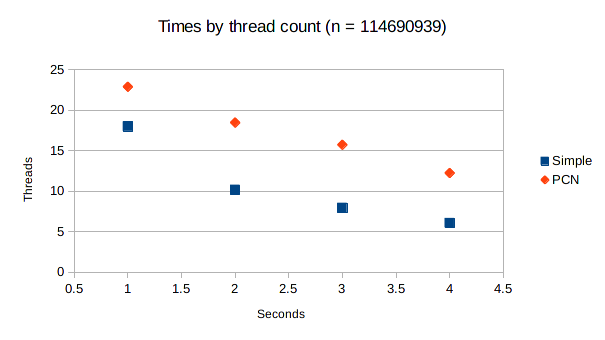
\includegraphics[width=\textwidth]{core_i5}
\end{frame}
\note{Here are some results from my own desktop compiled with GCC 4.8, and with 4 inputs and
outputs.
And as you can see the \lstinline|fetch_add| implementation actually scales fairly well,
and performs better than the counting network by around a factor of two.
I also tested sequential vs relaxed consistency but it made no noticeable difference.}


\begin{frame}
\frametitle{Results - Saturn}
\begin{itemize}
\item Compiled with g++-4.7, \lstinline|-std=gnu++11 -O3|
\item 48 inputs and outputs
\end{itemize}

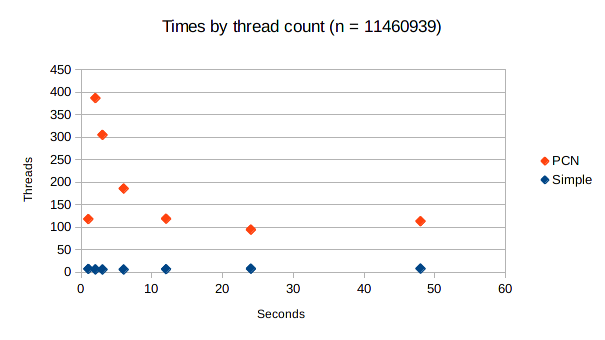
\includegraphics[width=\textwidth]{saturn}
\end{frame}
\note{I also benchmarked on the saturn system, this time with GCC 4.7 and 48 inputs and outputs.
There were a couple of differences; for instance, \lstinline|fetch_add| did not scale at all, with
times staying more or less constant.
The counting network was also much slower. Interestingy, the sequential implementation
was four times faster than using two threads. The best performance at around 24
processes was still ten times slower than the \lstinline|fetch_add| implementation.}

\begin{frame}
\frametitle{Reasons?}
\begin{itemize}
\item Valgrind shows nothing interesting, code seems to be sane.
\item Counting networks unsuited for this task (we don't return count after inc, thus
losing a major advantage).
\item Many! more instructions instead of a single \lstinline|fetch_add|.
\item No thread locality.
\end{itemize}
\end{frame}
\note{So what are the reasons for these results? Valgrind did not turn up any problems, so
the implementation seems to be sane.

One of the major advantages of counting networks is that each thread can arrive at the current count
at the end of an \lstinline|incr()| operation. Since these are not needed here, we could have just
created a single counter per thread instead of using a counting network.

Of course traversing a network uses many more instructions than simply doing a \lstinline|fetch_add|.

Finally, a counting network has very bad thread locality; most balancers could be used by
every thread at once.
}

\begin{frame}
\frametitle{THE END}
\end{frame}

\end{document}
